\documentclass[../main.tex]{subfiles}
\begin{document}
\chapter{Discrete Random Variables}
\section{Discrete Probability Distributions}
\subsection{Definition}
\begin{definition}[Discrete Probability Distribution]
  Suppose we have a probability space $(\Omega, \salg, \P)$ where $\Omega$ is \textbf{finite or countable}:
  \[
    \Omega = \{\omega_1, \omega_2, \ldots\},\ \salg = \powerset{\Omega}
  \]
  If we know $\P(\{\omega_i\})$ for all $i$, then for any $A \in \salg$:
  \[
    \P(A) = \P\left(\bigcup_{\omega_i \in A} \{\omega_i\}\right) = \sum_{\omega_i \in A} \P(\{\omega_i\})
  \]
  We then call $(\P(\{\omega_i\}))_i$ a \textit{discrete probability distribution} and we write $p_i = \P(\{\omega_i\})$.
\end{definition}
Since the $p_i$ are all probabilities, we must have $p_i \geq 0\ \forall i$.
Furthermore, since $\P(\Omega) = 1$, we must also have $\sum_{i} p_i = 1$
\begin{remark}[Summary]
   If we have a probability space $(\Omega, \salg, \P)$ where the $\Omega$ is at most countably infinite, then the \textit{discrete probability distribution} refers to the probabilities that $\P$ assigns to each singleton $\{\omega_i\}$ of $\Omega$.
\end{remark}
We will now cover some important discrete probability distributions.
\subsection{Bernoulli Distribution}
\label{bernoulliDist}
\begin{definition}[Bernoulli Distribution]
  The \textit{Bernoulli distribution} with parameter $p \in [0, 1]$, models a probability space with two outcomes where:
  \[
    \Omega = \{0, 1\},\ p_0 = \P(\{0\}) = 1 - p,\ p_1 = \P(\{1\}) = p
  \]
\end{definition}
This means Bernoulli distributions model the outcome of a single trial with two outcomes, for example the toss of a biased coin.
If we associate tails with 0 and heads with 1 then:
\[
  \P(\text{Heads}) = p_1 = p,\ \P(\text{Tails}) = p_0 = 1 - p
\]
\begin{remark}
  A coin with a probability $p$ of heads is sometimes called a $p$-coin.
\end{remark}
\subsection{Binomial Distribution}
\label{binomialDist}
\begin{definition}[Binomial Distribution]
  The \textit{binomial distribution} with parameters $n \in \N$ and $p \in [0, 1]$ is denoted $\binomial(n, p)$.

  It models number of successes in $n$ independent trials, each with an outcome of either success, with probability $p$, or failure, with probability $1 - p$.

  $\Omega$ all the possible numbers of trials where the outcome was success, i.e. $\Omega = \{1, \ldots, n\}$ as we can have anywhere from 1 to $n$ successful trials.

  The probability $p_k = \P(\{k\})$ is:
  \[
    p_k = \P(\text{$k$ successes}) = \binom{n}{k}p^{k}(1 - p)^{n - k} \text{ for $k \in \Omega$}
  \]
  as there are $\binom{n}{k}$ choices for when the successes should be.
\end{definition}
\begin{remark}[Intuition]
  We can think of the binomial distribution as modelling the number of heads we get if we toss a $p$-coin $n$ times.
\end{remark}
\subsection{Multinomial Distribution}
\begin{definition}[Multinomial Distribution]
  The \textit{multinomial distribution} with parameters $n \in \N$ and $p_1, \ldots, p_k \in [0, 1]$ such that $\sum_{i = 1}^{k} p_i = 1$, is denoted $\multinomial(n, p_1, \ldots, p_k)$.

  It models the outcome of $n$ independent trials, each with $k$ outcomes of probability $p_i$ for $1 \leq i \leq k$.

  $\Omega$ is the set of all tuples whose entries are the number of times $n_i$ each of the $k$ outcomes occurred:
  \[
    \Omega = \left\{(n_1, \ldots, n_k) \in \N^{k}_0 : \sum_{i = 1}^{k} n_i = n\right\}
  \]
  We require their sum to be $n$ as we did $n$ trials in total.

  The probability of a particular tuple, $p_{n_1, \ldots, n_k} = \P(\{(n_1, \ldots, n_k)\})$ is:
  \begin{align*}
    p_{n_1, \ldots, n_k} &= \binom{n}{n_1}p^{n_1}_{1} \cdot \binom{n - n_1}{n_2}p^{n_2}_{2} \cdots \binom{n - n_1 - \cdots - n_{k - 1}}{n_k} p^{n_k}_{k} \\
                         &= \binom{n}{n_1, \ldots, n_k} \cdot p^{n_1}_{1} \cdots p^{n_k}_{n}
  \end{align*}
  This uses the \textit{multinomial coefficient} that we saw in \cref{multinomialCoefficients}.
\end{definition}
\begin{remark}[Intuition]
  We can think of the multinomial distribution as modelling the results of tossing $n$ balls independently into $k$ boxes where each ball goes into box $i$ with probability $p_i$.
  Therefore:
  \[
    \P(n_1 \text{ balls in box 1}, \ldots, n_k \text{ balls in box $k$}) = p_{n_1, \ldots, n_k}
  \]
\end{remark}
\subsection{Geometric Distribution}
\begin{definition}[Geometric Distribution]
  The \textit{geometric distribution} with parameter $p \in [0, 1]$ is denoted $\geometric(p)$.
  There are two ways to define the geometric distribution:

  \textbf{Starting from 1}\par
    When starting from 1, it models the number of \textit{Bernoulli trials} (success with probability $p$, failure with probability $1 - p$) \textbf{needed to get the first success}.

    In this case $\Omega$ is the possible numbers of trials needed before a success first occurs so $\Omega = \N$.

    The probability $p_k = \P(\{k\})$ is then:
    \[
      p_k = \P(\text{$k$ trials needed for the first success}) = (1-p)^{k - 1}p \text{ for } k \in \Omega
    \]
  \textbf{Starting from 0}\par
    Starting from 0 is defined similarly, however, it now models the \textbf{number of failures before the first success}.
    So $\Omega$ is instead $\N_0$ and $p_k = \P(\{k\})$ is:
    \[
      p_k = \P(\text{$k$ failures before the first success}) = (1-p)^{k}p \text{ for } k \in \Omega
    \]
\end{definition}
\begin{remark}[Intuition]
  Consider tossing a $p$-coin until you get heads.
  We can think of the geometric distribution as modelling the number of tosses needed before the first head (if starting from 1), or the number of tails you would see before the first head (if starting from 0).
\end{remark}
\subsection{Poisson Distribution}
\begin{definition}[Poisson Distibution]
  The \textit{Poisson distribution} with parameter $\lambda > 0$ is denoted $\poisson(\lambda)$.

  It models the probability of a given number of events occurring in a fixed interval of time if these events occur with a mean rate $\lambda$ per time interval and independently of the time since the last event.

  $\Omega$ is all the possible numbers of times an event could occur in the interval, i.e., $\Omega = \N_0$.

  The probability $p_k = \P(\{k\})$ is:
  \[
    p_k = \P(\text{$k$ events in one interval}) = \frac{\lambda^{k} e^{-\lambda}}{k!}
  \]
\end{definition}
\begin{remark}
  Although we defined the Poisson distribution using an interval of time, it can also be used with over intervals such as areas or volumes.
\end{remark}
\begin{remark}[Intuition]
  Suppose customers arrive at a shop at a constant average rate of $\lambda$ customers per hour.
  We can think of the Poisson distribution as modelling the number of customers that arrive in a given hour, assuming that they arrive independently of each other and that customers cannot arrive at exactly the same instant.
\end{remark}
\subsubsection{Limit of a binomial distribution}
The Poisson distribution can be thought of as the limit of a binomial distribution (\cref{binomialDist}).

Suppose that the events occur in the interval $[0, 1]$.
We can discretise $[0, 1]$ as $[\frac{i - 1}{N}, \frac{i}{N}]$ for $i = 1, \ldots, N$ for some $N \in \N$.

In each interval $[\frac{i - 1}{N}, \frac{i}{N}]$, suppose the event occurs with probability $p$ and does not occur with probability $1 - p$ independently for different intervals.
\[
  \widetilde{p}_k = \P(\text{event occurred $k$ times}) = \binom{N}{k} p^{k} (1 - p)^{N - k},\ k = 0, \ldots, N
\]
as we pick a subset of $k$ intervals for the event to occur in.
This is $\binomial(N, p)$.

As $\lambda$ is the rate of the event occurring over $[0, 1]$, the probability of it occurring in one of the $N$ intervals is approximately $p = \frac{\lambda}{N}$.
Substituting this into $p_k$, we have:
\[
  \widetilde{p}_k = \frac{N!}{k!(N - k)!} \left(\frac{\lambda}{N}\right)^{k} \left(1-\frac{\lambda}{N}\right)^{N - k}
\]
Keeping $k$ fixed and taking the limit as $N \to \infty$ so that the intervals become infinitesimal and our approximation becomes exact:
\[
  \widetilde{p}_k = \frac{\lambda^{k}}{k!} \cancelto{1}{\frac{N(N - 1) \cdots (N - k + 1)}{N^{k}}} \cancelto{e^{-\lambda}}{\left(1 - \frac{\lambda}{N}\right)^{N - k}}
\]
So we see that $\widetilde{p}_k \to \frac{\lambda^{k} e^{-\lambda}}{k!} = p_k$ as $N \to \infty$.
\section{Random Variables}
\subsection{Definition}
Consider a probability space $(\Omega, \salg, \P)$:
\begin{definition}[Random Variable]
  A \textit{random variable} is a function $X: \Omega \to \R$ with the property that for $\forall x \in \R$:
  \[
    \{\omega \in \Omega : X(\omega) \leq x\} \in \salg
  \]
\end{definition}
We impose the restriction that $\{\omega \in \Omega : X(\Omega) \leq x\} \in \salg$ so that we are able to talk about the probability of it occurring as an event.
\begin{remark}[Notation]
  We write $\{X \leq x\} \equiv \{\omega \in \Omega: X(\omega) \leq x\}$ and for any $A \subseteq \R$, we write $\{X \in A\} \equiv \{\omega \in \Omega: X(\omega) \in A\}$.
\end{remark}
\begin{example}[Indicator Functions]
  Let $A \in \salg$.
  \label{indicatorFunction}
  Define the \textit{indicator} of $A$ as:
  \[
    1_A: \Omega \to \{0, 1\},\ 1_A(\omega) = \begin{cases}
      1 & \text{ if } \omega \in A \\
      0 & \text{ if } \omega \in A^{\comp}
    \end{cases}
  \]
  $1_A$ is a random variable as for $x \geq 1$, $\{\omega \in \Omega: 1_A(\omega) \leq x\} = \Omega \in \salg$, and for $x < 1$, $\{\omega \in \Omega: 1_A(\omega) \leq x\} = A^{\comp} \in \salg$ which is true as $A \in \salg$.
\end{example}
\begin{definition}[Probability Distribution Function]
  For a random variable $X$, we define the \textit{probability distribution function of $X$} to be:
  \[
    F_X: \R \to [0, 1],\  F_X(x) = \P(X \leq x)
  \]
\end{definition}
\begin{definition}[$n$-dimensional Random Variable]
  $X = (X_1, \ldots, X_n)$ is called a \textit{random variable in $\R^{n}$} if $(X_1, \ldots, X_n): \Omega \to \R^{n}$ such that $\forall x_1, \ldots, x_n \in \R$:
  \[
    \{\omega: X(\omega) \leq x_1, \ldots, X_n(\omega) \leq x_n\} \in \salg
  \]
  Equivalently, we require that all $X_i$ are real random variables so that:
  \[
    \{X_1 \leq x_1, \ldots, X_n \leq x_n\} = \{X_1 \leq x_1\} \cap \cdots \cap \{X_n \leq x_n\} \in \salg
  \]
  as $\{X_i \leq x_i\} \in \salg\ \forall i \in \{1, \ldots, n\}$ as all the $X_i$ are random variables.
\end{definition}
\begin{remark}[Notation]
  We write $\{X_1 \leq x_1, \ldots, X_n \leq x_n\} \equiv \{\omega: X(\omega) \leq x_1, \ldots, X_n(\omega) \leq x_n\}$.
\end{remark}
\subsection{Discrete Random Variables}
\begin{definition}[Discrete Random Variable]
  A random variable $X$ is called \textit{discrete} if it takes values in a countable set.

  Suppose it takes values in a countable set $S$, then for every $x \in S$, we write:
  We call $(p_x)_{x \in S}$ the \textit{probability mass function} or \textit{pmf} of $X$ or the \textit{distribution} of $X$.

\end{definition}
\begin{definition}[Probability Mass Function]
  For a discrete random variable $X$ taking values in a countable set $S$, the \textit{probability mass function}, \textit{pmf}, or \textit{distribution} of $X$ is defined to be:
  \label{pmf}
  \[
    p_X: X \to S,\ x \mapsto \P(X = x) = \P(\{\omega \in \Omega: X(\omega) = x\})\
  \]
  We also use the notation $p_x$ to mean $\P(X = x)$ if it is clear what distribution we are referencing.
\end{definition}
If $A \subseteq S$, then $\P(X \in A) = \sum_{x \in A} p_X(x)$.

If the $p_x$ are the Bernoulli distribution, then we say that $X$ is a \textit{Bernoulli r.v. (random variable)}, or we say that \textit{$X$ is Bernoulli distributed}.
For other discrete distributions, we use a similar convention, for example, we might say that $X$ is binomially distributed or that $X$ follows a Poisson distribution.
\begin{remark}[Notation]
  We use the notation $X \sim \binomial(n, p)$ to mean ``$X$ is binomially distributed'', and similarly for other distributions.
\end{remark}
\begin{remark}[Recap]
Recall from \cref{independentEvents} that two events $A, B \in \salg$ are independent if $\P(A \cap B) = \P(A)\P(B)$.
\end{remark}
\begin{definition}[Independent Discrete Random Variables]
  If $X_1, \ldots, X_n$ are discrete random variables with values in $S_1, \ldots, S_n$, then they are called \textit{independent random variables} if $\forall x_1 \in S_1, \ldots, x_n \in S_n$:
  \label{independentDiscreteRV}
  \[
    \P(X_1 = x_1, \ldots, X_n = x_n) = \P(X_1 = x_1) \cdots \P(X_n = x_n)
  \]
\end{definition}
This builds on our definition for independence of events.
For discrete random variables $X_1, X_2$, we using the events $\{X_1 = x_1\}$ and $\{X_2 = x_2\}$ but require that these events are independent \textbf{for all} possible $x_1 \in S_1$ and $x_2 \in S_2$.
If this is the case then:
\begin{align*}
  \P(X_1 = x_1, X_2 = x_2) &= \P(\{X_1 = x_1\} \cap \{X_2 = x_2\}) \\
                           &= \P(\{X_1 = x_1\})\P(\{X_2 = x_2\}) \text{ by independence of events} \\
                           &= \P(X_1 = x_1)\P(X_2 = x_2)
\end{align*}
for all $x_1 \in S_1$ and $x_2 \in S_2$.

\begin{lemma}
  If $X_1, X_2, X_3$ are independent discrete random variables, then $X_1$ is independent of $X_2$.
\end{lemma}
\begin{proof}
  We can rewrite $\P(X_1 = x_1, X_2 = x_2)$ as a countable sum over the possible values for $X_3$:
  \begin{align*}
    \P(X_1 = x_1, X_2 = x_2) &= \sum_{x_3} \P(X_1 = x_1, X_2 = x_2, X_3 = x_3) \\
                             &= \sum_{x_3} \P(X_1 = x_2)\P(X_2 = x_2)\P(X_3 = x_3) \\
                             &= \P(X_1 = x_1)\P(X_2 = x_2) \sum_{x_3} \P(X_3 = x_3) \\
                             &= \P(X_1 = x_1)\P(X_2 = x_2) \\
  \end{align*}
  Therefore, $X_1$ and $X_2$ are independent.
\end{proof}
\begin{lemma}
  If $X$ and $Y$ are independent discrete random variables and $g: \R \to \R$, then $g(X)$ and $Y$ are independent.
  \label{rvFunctionIndependence}
\end{lemma}
\begin{proof}
  We can partition $\{g(X) = w, Y = y\}$ up as:
  \begin{align*}
    \P(g(X) = w, Y = y) &= \sum_{x \in g^{-1}(\{w\})} \P(X = x, Y = y) \\
                        &= \sum_{x \in g^{-1}(\{w\})} \P(X = x)\P(Y = y) \text{ as $X \perp Y$}\\
                        &= \P(Y = y) \sum_{x \in g^{-1}(\{w\})} \P(X = x) \\
                        &= \P(Y = y)\P(g(X) = w)
  \end{align*}
  so $g(X) \perp Y$.
\end{proof}
\begin{example}
  \label{binomialAsBernSum}
  Consider tossing a $p$-coin $N$ times independently, as usual, we associate tails with 0 and heads with 1 so that $\Omega =\{0, 1\}^{N},\ \salg = \powerset{\Omega}$.
  For some $\omega \in \Omega$, label the elements of $\omega$ as $(\omega_1, \ldots, \omega_n)$ where $\omega_i$ is the outcome of the $i$-th toss.

  We calculate the probability of a singleton event $\{\omega\}$ as:
  \[
    p_\omega = \P(\{\omega\}) = \prod_{k = 1}^{N} p^{\omega_k} (1 - p)^{1 - \omega_k}
  \]
  The terms of the product give the correct probability for each toss as:
  \[
     p^{\omega_k} (1-p)^{1 - \omega_k}= \begin{cases}
     p & \text{ if } \omega_k = 1 \\
     1 - p & \text{ if } \omega_k = 0
    \end{cases}
  \]

  For all $\forall k = 1, \ldots, N$, define the random variables $X_k: \Omega \to \{0, 1\}$, $X_k(\omega) = \omega_k$.
  These are all random variable as for all $x \in \R$, $\{\omega \in \Omega: X_k(\omega) \leq x\} \in \powerset{\omega} = \salg$ and are all discrete r.v.s as they take values in the countable set $\{0, 1\}$.

  As these are independent tosses, for any $k$ (i.e. the $k$-th toss):
  \[
    \P(X_k = 1) = \P(\omega_k = 1) = p \text{ and } \P(X_k = 0) = \P(\omega_k = 0) = 1 - p
  \]
  So $X_k$ is Bernoulli r.v. (see \cref{bernoulliDist}) with parameter $p$.

  We can also show that $X_1, \ldots, X_n$ are independent r.v.s.
  For $\forall x_1, \ldots, x_N \in \{0, 1\}$:
  \begin{align*}
    \P(X_1 = x_1, \ldots, X_n = x_n) &= \P(\{(x_1, \ldots, x_n)\})\\
                                     &= \prod_{k = 1}^{N} p^{x_k}(1 - p)^{1 - x_k} \\
                                     &= \prod_{k = 1}^{N} \P(X_k = x_k)
  \end{align*}
  so they are independent.

  We can also define a new discrete random variable $S_N: \Omega \to \N_0$:
  \[
    S_N(\omega) = X_1(\omega) + \cdots + X_N(\omega) = \text{\#(heads in $n$ tosses)}
  \]
  this again has to be a random variable as $\salg = \powerset{\Omega}$.
  We then have:
  \[
    \P(S_N = k) = \binom{N}{k}p^{k}(1-p)^{N - k}
  \]
  which is $\binomial(N, p)$ so $S_N$ is a binomial r.v.
  So a binomial r.v. with parameters $N$ and $p$ can also be though of as the sum of $N$ Bernoulli r.v.s with parameter $p$.
\end{example}
\subsection{Expectation}
\begin{definition}[Non-negative Random Variable]
  Let $X: \Omega \to \R$ be a random variable.
  We say that $X$ is \textit{non-negative} if $X(\omega) \geq 0\ \forall \omega \in \Omega$.
\end{definition}
\begin{definition}[Expectation for non-negative discrete random variables]
  For a \textbf{non-negative discrete random variable} $X$, we define the \textit{expectation} of $X$ to be:
  \label{nonNegativeExpectation}
  \[
    \E[X] = \sum_{\omega \in \Omega} \P(\{\omega\})X(\omega)
  \]
  since $X$ is a discrete random variable, this is a finite or countable sum.
\end{definition}
Define $\Omega_X = \{X(\omega): \omega \in \Omega\}$, that is, the image of $\Omega$ under $X$.
This allows us to partition $\Omega$ into the disjoint sets $\{\omega \in \Omega: X(\omega) = x\} = \{X = x\}$ for each $x \in \Omega_x$.
We can therefore write $\Omega = \bigcup_{x \in \Omega_X} \{X = x\}$.
Since they are disjoint, we can rewrite $\E[X]$ as follows:
\label{expectationPartition}
\begin{align*}
  \E[X] &= \sum_{\omega \in \Omega} X(\omega) \P(\{\omega\}) \\
        &= \sum_{x \in \Omega_X} \sum_{\omega \in \{X = x\}} X(\omega)\P(\{\omega\}) \\
        &= \sum_{x \in \Omega_X} \sum_{\omega \in \{X = x\}} x \cdot \P(\{\omega\}) \text{ as $X(\omega) = x$ for $\omega \in \{X = x\}$} \\
        &= \sum_{x \in \Omega_X} x \sum_{\omega \in \{X = x\}} \P(\{\omega\}) \\
        &= \sum_{x \in \Omega_X} x \cdot \P(X = x) \text{ as $P(A) = \sum_{\omega \in A} \P(\{\omega\})$ for finite/countable $A$}
\end{align*}
So, the expectation of $X$ is a weighted average of the values taken by $X$ with weights given by $\P(X = x)$.
This formula for expectation is used more often than the one in the definition.
\begin{example}[Expectation of Binomial Distributed Variable]
  \label{binomialExpectation}
  Suppose $X \sim \binomial(N, p)$.
  This means that:
  \[
    \P(X = k) = \binom{N}{k}p^{k}(1-p)^{N-k}\ \forall k \in \{0, \ldots, N\}
  \]
  To find the expected value, $\Omega_X = \{0, \ldots, N\}$ so:
  \begin{align*}
    \E[X] &= \sum_{k = 0}^{N} k \cdot \P(X = k) \\
          &= \sum_{k = 1}^{N} k \cdot \frac{N!}{(N - k)!k!} p^{k}(1 - p)^{N - k}  \text{ discard first term as 0} \\
          &= Np \cdot \sum_{k = 1}^{N} \frac{(N - 1)!}{(k - 1)!((N - 1) - (k - 1))!}p^{k - 1}(1 - p)^{(N - 1) - (k - 1)} \\
          &= Np \cdot \sum_{k = 1}^{N} \binom{N-1}{k - 1}p^{k - 1}(1 - p)^{(N - 1) - (k - 1)} \\
          &= Np \cdot \sum_{k = 0}^{N - 1} \binom{N - 1}{k}p^{k}(1 - p)^{(N - 1) - k} \text{ re-indexing $k \mapsto k + 1$}\\
          &= Np (p + 1 - p)^{N - 1} = Np
  \end{align*}
  So the expected value of a random variable that is binomially distributed is the product of its parameters.
\end{example}
\begin{example}[Expectation of Poisson Distributed Variable]
  \label{poissonExpectation}
  Suppose $X \sim \poisson(\lambda)$, $\lambda > 0$.
  This means that:
  \[
    \P(X = k) = \frac{e^{-\lambda} \lambda^{k}}{k!}\ \forall k \in \N_0
  \]
  To find the expected value, $\Omega_X = \N_0$ so:
  \begin{align*}
    \E[X] &= \sum_{k = 0}^{\infty} k \cdot \P(X = k) \\
          &= \sum_{k = 1}^{\infty} k \cdot e^{-\lambda} \frac{\lambda^{k}}{k!} \text{ discard first terms as 0} \\
          &= e^{-\lambda} \lambda \sum_{k = 1}^{\infty} \frac{\lambda^{k - 1}}{(k - 1)!} \\
          &= e^{-\lambda} \lambda \sum_{k = 0}^{\infty} \frac{\lambda^{k}}{k!} \text{ re-indexing $k \mapsto k - 1$} \\
          &= e^{-\lambda} \lambda e^{\lambda} = \lambda
  \end{align*}
  So the expected value of a random variable that follows a Poisson distribution is just the value of the parameter $\lambda$.
\end{example}
\subsubsection{Expectation for possibly negative discrete random variables}
So far we have only defined expectation for \textbf{non-negative} discrete random variables in \cref{nonNegativeExpectation}.
However we would like this to extend this to r.v.s which can take negative values.
\begin{remark}[Notation]
  For any random variable $X$, define the random variables $X^{+} = \max\{X, 0\}$ and $X^{-} = \max\{-X, 0\}$.

  We can then write $X = X^{+} - X^{-}$ and $|X| = X^{+} + X^{-}$.
\end{remark}
Suppose $X$ is a discrete random variable.
We can find $\E[X^{+}]$ and $\E[X^{-}]$, since they are non-negative.
\begin{definition}[Expectation of a possibly negative discrete random variable]
  If at least one of $\E[X^{+}]$ and $\E[X^{-}]$ is finite, then we define the expectation of $X$ to be:
  \[
    \E[X] = \E[X^{+}] - \E[X^{-}]
  \]
  If both $\E[X^{+}]$ and $\E[X^{-}]$ are infinite, then $\E[X]$ is not defined.
  Whenever we write $\E[X]$, we imply that it is defined.
\end{definition}
When $\E[X]$ is well-defined, then we have the same formula as before:
\[
  \E[X] = \sum_{x \in \Omega_X} x \cdot \P(X = x)
\]
\begin{definition}[Integrable random variable]
  If $\E[|X|] < \infty$, then we say that $X$ is \textit{integrable}.
\end{definition}
\subsubsection{Properties of Expectation}
\begin{proposition}[Basic Properties of Expectation]
\label{expectationProperties}
\begin{enumerate}
  \item If $X \geq 0$, then $\E[X] \geq 0$
  \item If $X \geq 0$ and $\E[X] = 0$, then $\P(X = 0) = 1$.
  \item If $c \in \R$, then $\E[cX] = c\E[X]$ and $\E[c + X] = c + \E[X]$.
  \item If $X$ and $Y$ are integrable random variables, then:
    \[
      \E(X + Y) = \E(X) + \E(Y)
    \]
  \item Let $c_1, \ldots, c_n \in \R$ and $X_1, \ldots, X_n$ integrable random variables, then:
    \[
      \E\left[\sum_{i = 1}^{n} c_i X_i\right] = \sum_{i = 1}^{n} c_i \E[X_i]
    \]
    by combining \textbf{iii} and \textbf{iv}.
    We require that they are integrable so that there is not issues with adding infinities.
\end{enumerate}
\end{proposition}
\begin{proof}
  \begin{enumerate}
    \item The sum only consists of non-negative terms as $\P: \salg \to [0, 1]$ and $X \geq 0$.
    \item $\sum_{x \in \Omega_X} x \cdot \P(X = x) = 0 \implies x \cdot \P(X = x) = 0\ \forall x \implies \P(X = x) = 0\ \forall x \neq 0$.
      So $\P(\Omega) = \sum_{x \in \Omega_x} \P(X = x) = \P(X = 0) \implies \P(X = 0) = 1$.
    \item Let $Y(\omega) = cX(\omega)$.
      \begin{align*}
        \sum_{y \in \Omega_Y} y \cdot \P(Y = y) &= \sum_{x \in \Omega_X} cx \cdot \P(Y = cx) \\
                                                &= c \cdot \sum_{x \in \Omega_X} \P(X = x) = \E[X]
      \end{align*}
      as $\{Y = cx\} = \{\omega \in \Omega: cX(\omega) = cx\} = \{X = x\}$.

      Similarly, let $Z(\omega) = X(\Omega) + c$.
      \begin{align*}
        \sum_{z \in \Omega_Z} z \cdot \P(Z = z) &= \sum_{x \in \Omega_X} (x + c) \cdot \P(Z = x + c) \\
                                                &= \sum_{x \in \Omega_X} (x + c) \cdot \P(X = x) \text{ as $\{Z = x + c\} = \{X = x\}$} \\
                                                &= \sum_{x \in \Omega_X} x \cdot \P(X = x) + c\sum_{x \in \Omega_X} \P(X = x) \\
                                                &= \E(X) + c \P(\Omega) = \E(X) + c
      \end{align*}
    \item Let $Z(\omega) = X(\omega) + Y(\omega)$.
      \begin{align*}
        \E(Z) &= \sum_{x \in \Omega_X} \sum_{y \in \Omega_y} (x + y) \P(X = x, y = Y) \\
              &= \sum_{x \in \Omega_X} x \cdot \sum_{y \in \Omega_X} \P(X = x, y = Y) + \sum_{y \in \Omega_Y} y \cdot \sum_{x \in \Omega_X} \P(X = x, y = Y) \\
              &= \sum_{x \in \Omega_X} x \cdot \P(X = x) + \sum_{y \in \Omega_y} y \cdot \P(Y = y) \\
              &= \E[X] + \E[Y]
      \end{align*}
    \item Follows from using \textbf{iii} and induction with \textbf{iv}.
  \end{enumerate}
\end{proof}
\begin{remark}
  Property \textbf{iv} above leads to an alternative proof for \cref{binomialExpectation}.

  We saw in \cref{binomialAsBernSum} that we can express $X$ as $X = B_1 + \cdots B_N$ where $B_i$ are all independent Bernoulli r.v.s with parameter $p$.
  We find that the expectation of a Bernoulli r.v. is:
  \[
    \E[B_i] = 0 \cdot \P(B_i = 0) + 1 \cdot \P(B_i = 1) = p
  \]
  since $\Omega_{B_i} = \{0, 1\}$.
  The expectation of $X$ is then the sum of these expectations:
  \[
    \E[X] = \E\left[\sum_{i = 1}^{N} B_i\right] = \sum_{i = 1}^{N} \E[B_i] = \sum_{i = 1}^{N} p = Np
  \]
\end{remark}
\begin{lemma}[Countably Infinite Expectation Sum]
  If $X_1, X_2, \ldots$ are non-negative discrete r.v.s, then:
  \label{sumExpectationSwap}
  \[
    \E\left[\sum_{n = 1}^{\infty} X_n\right] = \sum_{n = 1}^{\infty} \E[X_n]
  \]
\end{lemma}
\begin{proof}
  $\Omega$ is countable as they are discrete random variables.
  \begin{align*}
    \E\left[\sum_{n = 1}^{\infty} X_n\right] &= \sum_{\omega \in \Omega} \left(\sum_{n = 1}^{\infty} X_n(\omega)\right)\P(\{\omega\}) \\
                                             &= \sum_{n = 1}^{\infty} \sum_{\omega \in \Omega} X_n(\omega)\P(\{\omega\}) \\
                                             &= \sum_{n = 1}^{\infty} \E[X_n]
  \end{align*}
  We are able to swap the two sums without issues as the terms are non-negative.
\end{proof}
\begin{example}[Expectation of Indicator Function]
  \label{expOfIndicator}
  Let $A \in \salg$ and $X(\omega) = 1_A(\omega)$.
  Calculating the expected value is easy as $\Omega_X = \{0, 1\}$ so:
  \begin{align*}
    \E[X] &= 0 \cdot \P(X = 0) + 1 \cdot \P(X = 1) \\
          &= \P(X = 1) \\
          &= \P(\{\omega \in \Omega: X(\omega) = 1_A(\omega) = 1\}) \\
          &= \P(A)
  \end{align*}
  So $\E[X] = \P(A)$.
\end{example}
\begin{proposition}[Expectation of a function of a r.v.]
  Let $g: \R \to \R$ and consider the discrete random variable $g(X)$ defined by $g(X)(\omega) = g(X(\omega))$.
  \label{expectationFunction}
  \[
    \E[g(X)] = \sum_{x \in \Omega_x} g(x) \cdot \P(X = x)
  \]
\end{proposition}
\begin{proof}
  Set $Y = g(X)$.
  \[
    \E[Y] = \sum_{y \in \Omega_Y} y \cdot \P(Y = y) \\
  \]
  We can rewrite the event $\{Y = y\}$ as:
  \begin{align*}
    \{Y = y\} &= \{\omega \in \Omega: Y(\omega) = y\} \\
              &= \{\omega \in \Omega: g(X(\omega)) = y\} \\
              &= \{\omega \in \Omega: X(\omega) \in g^{-1}(\{y\})\} \\
              &= \{X \in g^{-1}(\{y\})\}
  \end{align*}
  So:
  \begin{align*}
    \E[Y] &= \sum_{y \in \Omega_y} y \cdot \P(X \in g^{-1}(\{y\})) \\
          &= \sum_{y \in \Omega_y} y \cdot \sum_{x \in g^{-1}(\{y\})} \P(X = x) \\
          &= \sum_{y \in \Omega_y} \sum_{x \in g^{-1}(\{y\})} g(x) \cdot \P(X = x) \text{ as $g(x) = y\ \forall x \in g^{-1}(\{y\})$}
  \end{align*}
  The sets $g^{-1}(\{y\})$ for all $y \in \Omega_Y$ just define a partition of $\Omega_x$ so summing over all elements of all partition is equivalent to summing over $\Omega_X$.
  Thus:
  \[
    \E[Y] = \E[g(X)] = \sum_{x \in \Omega_X} g(x) \cdot \P(X = x)
  \]
\end{proof}
\begin{lemma}[Expectation of a discrete r.v. in $\N$]
  If $X$ is a discrete random variable that only takes values in $\N$, then:
  \[
    \E[X] = \sum_{k = 1}^{\infty} \P(X \geq k) = \sum_{k=0}^{\infty} \P(X > k)
  \]
\end{lemma}
\begin{proof}
  For any $n \in \N$:
  \[
    n = \sum_{k = 1}^{\infty} 1(n \geq k) = \sum_{k = 0}^{\infty} 1(n > k)
  \]
  As there are exactly $n$:
  \begin{itemize}
    \item $k \in \N$ such that $n \geq k$
    \item  $k \in \N_0$ such that $n > k$
  \end{itemize}
  Therefore, since $X(\omega) \geq 0$ and $X(\omega) \in \N$ for all $\omega$, we have the following:
  \[
    X(\omega) = \sum_{k = 1}^{\infty} 1(X(\omega) \geq k) = \sum_{k = 0}^{\infty} 1(X(\omega) > k)
  \]
  for all $\omega$.

  Taking the expectation, as they are non-negative, we can apply \cref{sumExpectationSwap}:
  \[
    \E[X] = \E\left[\sum_{k = 1}^{\infty} 1(X \geq k)\right] = \sum_{k = 1}^{\infty} \E[1(X \geq k)] = \sum_{k = 1}^{\infty} \P(X \geq k)
  \]
  using $\E[1_A] = \P(A)$ from \cref{expOfIndicator} and similarly for the sum starting from 0.
\end{proof}
\subsection{Indicator Functions}
We introduce the indicator in \cref{indicatorFunction} and found that $\E[1(A)] = \P(A)$ in \cref{expOfIndicator}.

There are a few useful properties of the indicator function:
\subsubsection{Properties of the Indicator}
\begin{enumerate}
  \item $1(A^{\comp}) = 1 - 1(A)$
  \item $1(A \cap B) = 1(A)1(B)$
  \item Since $(A \cup B)^{\comp} = A^{\comp} \cap B^{\comp}$:
    \begin{align*}
      1(A \cup B) &= 1 - 1((A^{\comp} \cap B^{\comp})) \\
                  &= 1 - (1 - 1(A))(1 - 1(B)) \\
                  &= 1(A) + 1(B) - 1(A)1(B)
    \end{align*}
\end{enumerate}
We can also use indicator functions to provide an alternative proof for the Principle of Inclusion Exclusion (\cref{inclusionExclusion}):
\subsubsection{Alternate proof for Inclusion Exclusion}
\begin{proof}
  We can extend property \textbf{iii} above to $n$ events $A_1, A_2, \ldots, A_n \in \salg$:
  \begin{align*}
    1(A_1 \cup \cdots \cup A_n) &= 1 - \prod_{i = 1}^{n} (1 - 1(A_i)) \\
                                &= \sum_{i = 1}^{n} 1(A_i) - \sum_{i_1 < i_2} 1(A_{i_1} \cap A_{i_2}) + \cdots + (-1)^{n + 1}1(A_1 \cap \cdots \cap A_n) \\
                                &= \sum_{k = 1}^{n} (-1)^{k + 1} \sum_{1 \leq i_1 < \ldots < i_k \leq n} 1(A_{i_1} \cap \cdots \cap A_{i_k})
  \end{align*}
  If we take expectations of both sides, we can split the expectation up using \cref{expectationProperties} and then use $\E[1(A)] = \P(A)$:
  \[
    \P(A_1 \cup \cdots \cup A_n) = \sum_{k = 1}^{n} (-1)^{k + 1} \sum_{1 \leq i_1 < \ldots < i_k \leq n} \P(A_{i_1} \cap \cdots \cap A_{i_k})
  \]
  which is the desired result:
\end{proof}
\subsection{Variance}
\begin{definition}[$r$-th moment]
  We call $\E[X^{r}]$ (provided it is well defined), the \textit{$r$-th moment of $X$}.
\end{definition}
\begin{remark}
  Expectation is then the \textit{first moment of $X$}.
\end{remark}
\begin{definition}[Variance]
  The \textit{variance} of $X$ is defined to be:
  \[
    \Var(X) = \E[(X - \E[X])^2]
  \]
\end{definition}
\begin{remark}[Intuition]
  The \textit{variance} is a measure of how well concentrated $X$ is around its expectation.
  The smaller the variance, the more concentrated $X$ is around its expectation.
\end{remark}
\begin{definition}[Standard-Deviation]
  The \textit{standard deviation} of $X$ is defined to be $\sqrt{\Var(X)}$.

\end{definition}
\begin{remark}[Notation]
  Standard deviation is often denoted as $\sigma$ and so the variance is sometimes written as $\sigma^2$.
\end{remark}
\begin{proposition}[Properties of Variance]
  \begin{enumerate}
    \item $\Var(X) \geq 0$
    \item If $\Var(X) = 0$, then $\P(X = \E[X]) = 1$.
    \item If $c \in \R$, then $\Var(cX) = c^2 \Var(X)$ and $\Var(X + c) = \Var(X)$
    \item $\Var(X) = \E[X^2] - (\E[X])^2$
    \item $\Var(X) = \min\limits_{c \in \R} \E[(X - c)^2]$ and the minimum is attained when $c = \E[X]$.
  \end{enumerate}
\end{proposition}
\begin{proof}
\begin{enumerate}
  \item $(X - \E[X])^2 \geq 0$ so by \cref{expectationProperties} \textbf{i}, $\Var(X) \geq 0$.
  \item $(X - \E[X])^2 \geq 0$ so by \cref{expectationProperties} \textbf{ii}, $\Var(X) = \E[(X - \E[X])^2] = 0 \implies \P(X = \E[X]) = 1$.
  \item
    Using \cref{expectationProperties} \textbf{iii}, we have:
    \begin{align*}
      \Var(cX) &= \E[(cX - \E[cX])^2] \\
               &= \E[c^2(X - \E[X])2] \\
               &= c^2 \E[(X - \E[X])^2] = c^2 \Var(X)
    \end{align*}
    Similarly:
    \begin{align*}
      \Var(c + X) &= \E[((c + X) - \E[c + X])^2] \\
                  &= \E[(c + X - c - \E[X])^2] \\
                  &= \E[(X - \E[X])^2] = \Var(X)
    \end{align*}
  \item We can expand the expectation as:
    \begin{align*}
      \Var(X) &= \E[X^2 - 2X\E[X] + (\E[X])^2] \\
              &= \E[X^2] - 2\E[X]\E[X] + (\E[X])^2 \\
              &= \E[X^2] - (\E[X])^2
    \end{align*}  %TODO note above positive
  \item Define the function $f(c) = \E[(X - c)^2]$.
    \begin{align*}
      f(c) &= \E[X^2 - 2cX + c^2] \\
           &= \E[X^2] - 2c\E[X] + c^2 \\
      \implies \deriv{f}{c} &= -2\E[X] + 2c
    \end{align*}
    So $\min\limits_{c \in \R}f(c) = f(\E(X)) = \E[(X - \E[X])^2] = \Var(X)$.
\end{enumerate}
\end{proof}
\begin{example}
  \label{varianceExample}
  \begin{enumerate}
    \item For $X \sim \binomial(n, p)$.
      We saw earlier in \cref{binomialExpectation} that $\E[X] = np$.
      It is easier if we rewrite $\Var(X)$ as:
      \begin{align*}
        \Var(X) &= \E[X^2 - X + X] - (\E[X])^2 \\
                &= \E[X(X - 1)] + \E[X] - (\E[X])^2
      \end{align*}
      Using \cref{expectationFunction}, we have:
      \begin{align*}
        \E[X(X-1)] &= \sum_{k = 2}^{n} k(k - 1) \frac{n!}{k!(n - k)!} p^{k}(1 - p)^{n - k} \\
                   &= (n - 1)n\sum_{k = 2}^{n} \frac{(n - 2)!}{(k - 2)!((n - 2) - (k - 2))!} p^{k}(1 - p)^{n - k} \\
                   &= (n - 1)np^2 \sum_{k = 2}^{n} \binom{n - 2}{k - 2}p^{k - 2}(1 - p)^{n - 2 - (k - 2)} \\
                   &= (n - 1)np^2 \sum_{k = 0}^{n - 2} \binom{n - 2}{k}p^{k}(1 - p)^{n - 2 - k} \text{ re-indexing $k \mapsto k + 2$}\\
                   &= (n - 1)np^2 (p + 1 - p)^{n - 2} \\
                   &= (n - 1)np^2
      \end{align*}
      and so:
      \[
        \Var(X) = (n - 1)np^2 + np - (np)^2 = np(1- p)
      \]
    \item For $X \sim \poisson(\lambda)$.
      We saw earlier \cref{poissonExpectation} that $\E[X] = \lambda$.
      Using the same trick as above, we have:
      \begin{align*}
        \E[X(X - 1)] &= \sum_{k = 2}^{\infty} k(k - 1)e^{-\lambda} \frac{\lambda^{k}}{k!} \\
                     &= e^{-\lambda} \lambda^2 \sum_{k = 2}^{\infty} \frac{\lambda^{k - 2}}{(k - 2)!} \\
                     &= e^{-\lambda} \lambda^2 e^{\lambda} = \lambda^2
      \end{align*}
      and so:
      \[
        \Var(X) = \lambda^2 + \lambda - \lambda^2 = \lambda
      \]
  \end{enumerate}
\end{example}
\subsection{Covariance}
\begin{definition}[Covariance]
  For random variables $X$ and $Y$, we define their \textit{covariance} to be:
  \[
    \Cov(X, Y) = \E[(X - \E[X])(Y - \E[Y])]
  \]
\end{definition}
\begin{remark}[Intuition]
  The \textit{covariance} is a measure of ``how independent'' $X$ and $Y$ are.
\end{remark}
\begin{proposition}[Properties of Covariance]
  \label{covarianceProperties}
  \begin{enumerate}
    \item $\Cov(X, Y) = \Cov(Y, X)$.
    \item $\Cov(X, X) = \Var(X)$.
    \item $\Cov(X, Y) = \E[XY] - \E[X]\E[Y]$
    \item Let $c \in \R$, then $\Cov(cX, Y) = c\Cov(X, Y)$ and $\Cov(c + X, Y) = \Cov(X, Y)$
    \item $\Var(X + Y) = \Var(X) + \Var(Y) + 2\Cov(X, Y)$
    \item For random variables $X, Y, Z$:
      \[
        \Cov(X + Y, Z) = \Cov(X, Z) + \Cov(Y, Z)
      \]
    \item More generally, for $\forall c_1, \ldots, c_n, d_1, \ldots, d_n \in \R$ and random variables $X_1, \ldots, X_n, Y_1, \ldots, Y_n$:
      \[
        \Cov\left(\sum_{i = 1}^{n} c_iX_i, \sum_{i = 1}^{n} d_i Y_i\right) = \sum_{i, j = 1}^{n} c_id_j \Cov(X_i, Y_i)
      \]
    \item For random variables $X_1, \ldots, X_n$:
      \[
        \Var\left(\sum_{i = 1}^{n} X_i\right) = \sum_{i = 1}^{n} \Var(X_i) + \sum_{i \neq j} \Cov(X_i, X_j)
      \]
  \end{enumerate}
\end{proposition}
\begin{proof}
  \begin{enumerate}
    \item Follows immediately from the definition.
    \item $\Cov(X, X) = \E[(X - \E[X])^2] = \Var(X)$.
    \item We can expand the covariance as:
      \begin{align*}
        \Cov(X, Y) &= \E[XY - Y\E[X] - X\E[Y] + \E[X]\E[Y]] \\
                   &= \E[XY] - \E[Y]\E[X] - \E[X]\E[Y] + \E[X]\E[Y] \\
                   &= \E[XY] - \E[X]\E[Y]
      \end{align*}
    \item Using \textbf{iii} and \cref{expectationProperties}:
      \[
        \Cov(cX, Y) = \E[cXY] - \E[cX]\E[Y] = c(\E[XY] - \E[X]\E[Y]) = c\Cov(X, Y)
      \]
      Similarly:
      \begin{align*}
        \Cov(c + X, Y) &= \E[XY + cY] - (\E[X] + c)\E[Y] \\
                       &= \E[XY] + c\E[Y] - \E[X]\E[Y] - c\E[Y] \\
                       &= \E[XY] - \E[X]\E[Y] = \Cov(X, Y)
      \end{align*}
    \item We can expand the variance as:
      \begin{align*}
        \Var(X + Y) &= \E[((X + Y) - \E[X + Y])^2] \\
                    &= \E[((X - \E[X]) + (Y - \E[Y]))^2] \\
                    &= \E[(X - \E[X])^2] + 2\E[(X - \E[X])(Y - \E[Y])] + \E[(Y - \E[Y])^2] \\
                    &= \Var(X) + 2\Cov(X, Y) + \Var(Y)
      \end{align*}
    \item We can expand this as:
      \begin{align*}
        \Cov(X + Y, Z) &= \E[(X + Y - \E[X + Y])(Z - \E[Z])] \\
                       &= \E[((X - \E[X]) + (Y - \E[Y]))(Z - \E[Z])] \\
                       &= \E[(X - \E[X])(Z - \E[Z])] + \E[(Y - \E[Y])(Z - \E[Z])] \\
                       &= \Cov(X, Z) + \Cov(Y, Z)
      \end{align*}
    \item Follows from \textbf{iv} and induction using \textbf{vi}.
    \item Using \textbf{ii} and \textbf{vii}:
      \begin{align*}
        \Var\left(\sum_{i = 1}^{n} X_i\right) &= \Cov\left(\sum_{i = 1}^{n} X_i, \sum_{i = 1}^{n} X_i\right) \\
                                              &= \sum_{i, j = 1}^{n} \Cov(X_i, X_j) \\
                                              &= \sum_{i = 1}^{n} \Cov(X_i, X_i) + \sum_{i \neq j}^{n} \Cov(X_i, X_j) \\
                                              &= \sum_{i = 1}^{n} \Var(X_i) + \sum_{i \neq j}^{n} \Cov(X_i, X_j)
      \end{align*}
  \end{enumerate}
\end{proof}
\begin{remark}[Recap]
  Recall from \cref{independentDiscreteRV} that if $X_1, \ldots, X_n$ are discrete random variables, then they are called \textit{independent} if $\forall x_1, \ldots, x_n$:
  \[
    \P(X_1 = x_1, \ldots, X_n = x_n) = \prod_{i = 1}^{n} \P(X_i = x_i)
  \]
\end{remark}
\begin{lemma}[Expectation of Product]
  Let $X$ and $Y$ be two independent random variables and let $f, g: \R \to \R^{+}$ then:
  \label{expectationProduct}
  \[
    \E[f(X)g(Y)] = \E[f(X)]\E[g(Y)]
  \]
\end{lemma}
\begin{proof}
  Let $Z = (X, Y)$ and define $h(Z) = f(X)g(Y)$.
  Using \cref{expectationFunction}, we have:
  \begin{align*}
    \E(h(Z)) &= \sum_{(x, y)} h(x, y)\P(Z = (x, y)) \\
             &= \sum_{(x, y)} f(X)g(Y)\P(X = x, Y = y) \\
             &= \sum_{(x, y)} f(X)g(Y)\P(X = x)\P(Y = y) \text{ as $X \perp Y$}\\
             &= \left[\sum_{x} f(X)\P(X = x)\right]\left[\sum_{y} g(Y)\P(Y = y)\right] \\
             &= \E[f(X)]\E[g(Y)]
  \end{align*}
  Thus $\E[f(X)g(Y)] = \E[h(Z)] = \E[f(X)]\E[g(Y)]$.
\end{proof}
\begin{corollary}
  If $X$ and $Y$ are independent, then $\Cov(X, Y) = 0$.
\end{corollary}
\begin{proof}
  The covariance of $X$ and $Y$ is just the product of two functions of $X$ and $Y$ so:
  \begin{align*}
    \Cov(X, Y) &= \E[(X - \E[X])(Y - \E[Y])] \\
               &= \E[X - \E[X]]\E[Y - \E[Y]] \\
               &= (\E[X] - \E[X])(\E[Y] - \E[Y]) \\
               &= 0
  \end{align*}
\end{proof}
\begin{corollary}
  If $X$ and $Y$ are independent random variables, then $\Var(X + Y) = \Var(X) + \Var(Y)$.
\end{corollary}
\begin{proof}
  $X \perp Y$ so $\Cov(X, Y) = 0$.
  Using \cref{covarianceProperties} \textbf{v}:
  \[
    \Var(X + Y) = \Var(X) + \Var(Y) + 2\Cov(X, Y) = \Var(X) + \Var(Y)
  \]
\end{proof}
\begin{corollary}
  If $X_1, \ldots, X_n$ are independent random variables then $\Var(\sum_{i = 1}^{n} X_i) = \sum_{i = 1}^{n} \Var(X_i)$.
\end{corollary}
\begin{proof}
  Using \cref{covarianceProperties} \textbf{vii}:
  \begin{align*}
    \Var\left(\sum_{i = 1}^{n} X_i\right) &= \sum_{i = 1}^{n} \Var(X_i) + \sum_{i \neq j}^{n} \Cov(X_i, X_j) \\
                                          &= \sum_{i = 1}^{n} \Var(X_i)
  \end{align*}
  Since $\Cov(X_i, X_j) = 0$ for $i \neq j$ as the $X_i$ are independent.
\end{proof}
\begin{remark}
  $\Cov(X, Y) = 0 \centernot \implies$ $X$ and $Y$ are independent.

  For example, let $X_1, X_2, X_3$ be independent Bernoulli random variables with parameter $\frac{1}{2}$ and recall that $\E[X_i] = \frac{1}{2}$.

  Set $Y_1 = 2X_1 - 1$, $Y_2 = 2X_2 - 1$, $Z_1 = Y_1 X_3$, and $Z_2 = Y_2 X_3$.
  We then have
  \[
    \E[Y_1] = \E[Y_2] = 2\left(\frac{1}{2}\right) - 1 = 0
  \]
  and
  \[
    \E[Z_1] = \E[Y_1 X_3] = \E[Y_1]\E[X_3] = 0
  \]
  so by the same argument $\E[Z_2] = 0$.

  So $\Cov(Z_1, Z_2) = \E[Z_1Z_2] - \cancelto{0}{\E[Z_1]\E[Z_2]} = \E[Y_1 Y_2 X^2_3] = \E[Y_1]\E[Y_2]\E[X^2_3] = 0$.
  Thus the covariance of $Z_1$ and $Z_2$ is 0.

  However, $Z_1$ is not independent of $Z_2$ since:
  \[
    \P(Z_1 = 0, Z_2 = 0) = \P(X_3 = 0) = \frac{1}{2}
  \]
  but:
  \[
    \P(Z_1 = 0) = \P(Z_2 = 0) = \frac{1}{2} \implies \P(Z_1 = 0)\P(Z_2 = 0) = \frac{1}{4} \neq \frac{1}{2}
  \]
  so $Z_1$ and $Z_2$ are not independent, despite having 0 covariance.
\end{remark}
\begin{example}
  Take $S_n \sim \binomial(n, p)$.
  From \cref{binomialAsBernSum}, we saw that we can express $S_n$ as a sum of independent Bernoulli random variables with parameter $p$:
  \[
    S_n = X_1 + \cdots + X_n
  \]
  For each Bernoulli random variable:
  \[
    \Var(X_i) = \E[X^2] - (\E[X])^2 = \E[X] - (\E[X])^2 = p - p^2 = p(1 - p)
  \]
  as $X^2 = X$ since $X \in \{0, 1\}$.

  We can therefore find $\Var(S_n)$ using:
  \[
    \Var(S_n) = \sum_{i = 1}^{n} \Var(X_i) = np(1-p)
  \]
  which agrees with the result from \cref{varianceExample}.
\end{example}
\section{Probabilistic Inequalities}
\subsection{Markov's Inequality}
\begin{proposition}[Markov's Inequality]
  If $X$ is a non-negative random variable and $a > 0$, then $\P(X \geq a) \leq \frac{\E[X]}{a}$.
\end{proposition}
\begin{proof}
  We have that:
  \[
    X \geq a \cdot 1(X \geq a)
  \]
  as either $X \geq a$, in which case $X \geq a \cdot 1$ which is true, or $X < a$, in which case $X \geq a \cdot 0 = 0$, which is also true.
  Taking expectations and using \cref{expOfIndicator} we get that:
  \[
    \E[X] \geq a \cdot \P(X \geq a)
  \]
  and the result follows.
\end{proof}
\subsection{Chebyshev's Inequality}
\begin{proposition}[Chebyshev's Inequality]
  If $X$ is a random variable with $\E[X] < \infty$, then $\forall a > 0$:
  \[
    \P(|X - \E[X]| \geq a) \leq \frac{\Var(X)}{a^2}
  \]
\end{proposition}
\begin{proof}
  \begin{align*}
    \P(|X - \E[X]| \geq a) &= \P(|X - \E[X]|^2 \geq a^2) \\
                           &\leq \frac{\E[(X - \E[X])^2]}{a^2} \text{ by Markov's Inequality} \\
                           &= \frac{\Var(X)}{a^2}
  \end{align*}
\end{proof}
\subsection{Cauchy-Schwarz Inequality}
\begin{proposition}[Cauchy-Schwarz Inequality]
  If $X$ and $Y$ are discrete random variables, then:
  \[
    \E[|XY|] \leq \sqrt{\E[X^2]\E[Y^2]}
  \]
\end{proposition}
\begin{proof}
  If both $\E[X^2]$ and $\E[Y^2]$ are infinite, then there is nothing to prove so assume that that $\E[X^2] < \infty$ and $\E[Y^2] < \infty$.

  In this case, we can check that $\E[|XY|]$ is also finite
  \[
    |XY| \leq \frac{1}{2}(X^2 + Y^2) \implies \E[|XY|] \leq \frac{1}{2}(\E[X^2] + \E[Y^2]) < \infty
  \]
  If $\E[X^2] = 0$ or $\E[Y^2] = 0$, then at least one of $X$ or $Y$ would have to be identically 0 so there would be nothing left to prove so assume that $\E[X^2] > 0$ and $\E[Y^2] > 0$.
  Since we have $|XY|$, $X^2$ and $Y^2$, it is also enough to show that this holds for $X, Y \geq 0$.

  Let $t \in \R$ and consider the random variable $(X - tY)^2$.
  Since this is non-negative, $\E[(X - tY)^2] \geq 0$ and so:
  \[
    \E[(X - tY)^2] = \E[X^2] - 2t\E[XY] + t^2 \E[Y^2] \geq 0
  \]
  We know wish to find some $t$ which leads to the inequality.
  To do this, let $f(t) = \E[X^2] -2t\E[XY] + t^2 \E[Y^2]$.
  We then have $f'(t) = -2\E[XY] + 2t\E[Y^2]$ and so the minimum of $f(t)$ is attained at $t_{*} = \frac{\E[XY]}{\E[Y^2]}$.
  Evaluating $f$ at $t_{*}$, we must get a non-negative value so:
  \[
    \E[X^2] - 2 \frac{(\E[XY])^2}{\E[Y^2]} + \frac{(\E[XY])^2}{\E[Y^2]} \geq 0 \implies (\E[XY])^2 \leq \E[X^2]\E[Y^2]
  \]
\end{proof}
\begin{lemma}
  We get equality in Cauchy-Schwarz if and only if one random variable is a constant multiple of the other.
\end{lemma}
\begin{proof}
  \begin{proofdirection}{Assume we have equality}
    $\E[|XY|] = \sqrt{\E[X^2]\E[Y^2]}$ so must have $f(t_*) = 0$, therefore:
    \begin{align*}
      f(t_*) = \E[(X - t_*Y)^2] = 0 \implies& \P(X - t_*Y = 0) = 1 \\
      \implies& \P(X = t_*Y) = 1
    \end{align*}
    So $X$ is a constant multiple of $Y$.
  \end{proofdirection}
  \begin{proofdirection}{Assume one is a multiple of the other}
    For the converse, if $X = cY$, then:
    \[
      \E[|XY|] = |c|\E[Y^2] = \sqrt{c^2\E[Y^2]^2} = \sqrt{c^2\E[Y^2]\E[Y^2]} = \sqrt{\E[X^2]\E[Y^2]}
    \]
  \end{proofdirection}
\end{proof}
\subsection{Jensen's Inequality}
\begin{definition}[Convex Function]
  A function $f: \R \to \R$ is called \textit{convex} if $\forall x, y \in \R$ and $\forall t \in [0, 1]$:
  \[
    f(tx + (1 - t)y) \leq tf(x) + (1 - t)f(y)
  \]
\end{definition}
That is, a function is convex if it lies below the chord between any two points on the curve:
\begin{center}
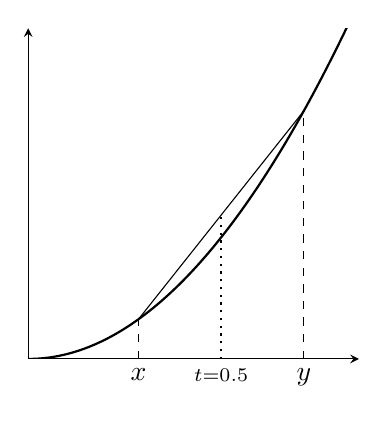
\begin{tikzpicture}[>=stealth, scale=1.4]
  \draw[->] (0, 0) -- (0, 3);
  \draw[->] (0, 0) -- (3, 0);

  \begin{scope}
    \clip (0, 0) rectangle (3, 3);
    \draw[thick, domain=0:3, smooth, samples=100] plot (\x,{(0.6 * \x)^2});
  \end{scope}
  \draw[dashed] (1, 0) node[below] {$x$} -- (1, 0.36);
  \draw[dashed] (2.5, 0) node[below] {$y$} -- (2.5, 2.25);
  \draw[dotted, thick] (1.75, 0) node[below] {$\scriptstyle t = 0.5$} -- (1.75, 1.3);
  \draw (1, 0.36) -- (2.5, 2.25);
\end{tikzpicture}
\end{center}
\begin{lemma}
  Let $f: \R \to \R$ be a convex function.
  $f$ is the supremum of all the lines lying below it.
  That is, $\forall m \in \R,\ \exists a, b \in \R$ such that:
  \label{convexLemma}
  \[
    f(m) = am + b \text{ and } f(x) \geq ax + b\ \forall x
  \]
  So the entire curve lies above the tangent at a given point:
  \begin{center}
  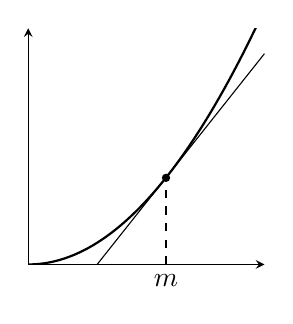
\begin{tikzpicture}[>=stealth]
    \draw[->] (0, 0) -- (0, 3);
    \draw[->] (0, 0) -- (3, 0);

    \begin{scope}
      \clip (0, 0) rectangle (3, 3);
      \draw[thick, domain=0:3, smooth, samples=100] plot (\x,{(0.6 * \x)^2});
    \end{scope}
    \draw (0.875, 0) -- (3, 2.677);
    \draw[dashed] (1.75, 0) node[below] {$m$} -- (1.75, 1.10);
    \fill (1.75, 1.10) circle (1.5pt);
  \end{tikzpicture}
  \end{center}
\end{lemma}
\begin{proof}
  Let $m \in \R$ and $x < m < y$.
  To use convexity, since $x < m < y$, we can write:
  \[
    m = tx + (1 - t)y
  \]
  for some $t \in [0, 1]$.
  Rearranging, we also have:
  \[
    t(m - x) = (1 - t)(y - m)
  \]
  Using convexity:
  \[
    f(m) = f(tx + (1 - t)y) \leq tf(x) + (1 - t)f(y)
  \]
  We can then rearrange and use the above equality:
  \begin{align*}
    t(f(m) - f(x)) &\leq (1 - t)(f(y) - f(m)) \\
    t(m - x)(f(m) - f(x)) &\leq (1 - t)(m - x)(f(y) - f(m)) \\
    (1 - t)(y - m)(f(m) - f(x)) &= (1 - t)(m - x)(f(y) - f(m)) \\
    \frac{f(m) - f(x)}{m - x} &\leq \frac{f(y) - f(m)}{y- m}
  \end{align*}
  Since this is for any $m$, this tells us that the slope at $y$ is grater than the slope at $x$:
  \begin{center}
  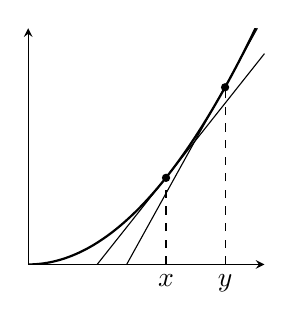
\begin{tikzpicture}[>=stealth]
    \draw[->] (0, 0) -- (0, 3);
    \draw[->] (0, 0) -- (3, 0);

    \begin{scope}
      \clip (0, 0) rectangle (3, 3);
      \draw[thick, domain=0:3, smooth, samples=100] plot (\x,{(0.6 * \x)^2});
    \end{scope}
    \draw (0.875, 0) -- (3, 2.677);
    \draw[dashed] (1.75, 0) node[below] {$x$} -- (1.75, 1.10);
    \fill (1.75, 1.10) circle (1.5pt);

    \draw (1.25, 0) -- (2.91, 3);
    \draw[dashed] (2.5, 0) node[below] {$y$} -- (2.5, 2.25);
    \fill (2.5, 2.25) circle (1.5pt);
  \end{tikzpicture}
  \end{center}
  Let $a = \sup\limits_{x < m}\frac{f(m) - f(x)}{m - x}$ and so $\frac{f(m) - f(x)}{m - x} \leq a$ $\forall x < m$.

  Combining this with the other inequality, $\forall x < m < y$:
  \[
    \frac{f(m) - f(x)}{m - x} \leq a \leq \frac{f(y) - f(m)}{y - m}
  \]
  If $z < m$, then we use the left hand inequality to yield $f(z) \geq a(z - m) + f(m)$.
  If $z > m$, then we use the right hand inequality to yield the same result.
  Therefore, $f(z) \geq az + (f(m) - am)\ \forall z$ and we get equality when $z = m$, as required.
\end{proof}
\begin{proposition}[Jensen's Inequality]
  Let $X$ be a random variable and $f: \R \to \R$ a convex function.
  \[
    \E[f(X)] \geq f(\E[X])
  \]
\end{proposition}
\begin{proof}
  Let $m = \E[X]$, as $f$ is convex, by \cref{convexLemma}, $\exists a, b \in \R$ such that:
  \[
    f(m) = am + b \text{ and } f(x) \geq ax + b\ \forall x
  \]
  Thus $f(X) \geq aX + b$, so taking expectations of both sides:
  \[
    \E[f(X)] \geq a\E[X] + b = am + b = f(m) = f(\E[X])
  \]
  as taking expectations preserves inequalities.
\end{proof}
\begin{remark}[Memorisation]
  To remember which way the inequality goes, consider $f(x) = x^2$.
  We already know that $\Var(X) = \E[X^2] - (\E[X])^2 \geq 0$ so we need $\E[X^2] \geq (\E[X])^2$ in Jensen's Inequality.
\end{remark}
\subsubsection{Cases of equality in Jensen's Inequality}
Let $f: \R \to \R$ be convex with the extra property that for $m = \E[X]$, $\exists a, b \in \R$ such that:
\[
  f(m) = am + b \text{ and } f(x) > ax + b\ \forall x \neq m
\]
What should $X$ satisfy so that $\E[f(X)] = f(\E[X])$?
We have that $f(X) \geq aX + b \implies f(X) - (aX + b) \geq 0$ so we can construct a new non-negative random variable $f(X) - (aX + b)$.

Taking expectations, we have:
\[
  \E[f(X)] \geq a \E[X] + b = am + b = f(m) = f(\E[X])
\]
We want $\E[f(X)] = f(\E[X])$ so this forces $\E[f(X)] = a \E[X] + b = \E[aX + b]$ and so:
\begin{align*}
  \E[f(X) - (aX + b)] = 0 &\implies \P(f(X) = aX + b) = 1 \\
\end{align*}
Since under our new restrictions, $f(x) = ax + b$ if only if $x = m = \E[X]$ so $\P(f(X) = aX + b) = 1 \implies \P(X = \E[X]) = 1$.
\begin{corollary}
  If $f$ be a convex function, then $\forall x_1, \ldots, x_n \in \R$:
  \label{jensenCorollary}
  \[
    \frac{1}{n} \sum_{k = 1}^{n} f(x_k) \geq f\left(\frac{1}{n}\sum_{k = 1}^{n} x_k\right)
  \]
\end{corollary}
\begin{proof}
  Let $X$ be a discrete random variable taking values from $\{x_1, \ldots, x_n\}$ with $\P(X = x_i) = \frac{1}{n}$.
  We can use \cref{expectationFunction} to find $\E[f(X)]$:
  \[
    \E[f(X)] = \sum_{k = 1}^{n} f(x_k)\P(X = x_k) = \frac{1}{n}\sum_{k = 1}^{n} f(x_k)
  \]
  We also have $\E[X] = \frac{1}{n}\sum_{k = 1}^{n} f(x_k)$ and as $f$ is convex $\E[f(X)] \geq f(\E[X])$, so:
  \[
    \frac{1}{n} \sum_{k = 1}^{n} f(x_k) \geq f\left(\frac{1}{n}\sum_{k = 1}^{n} x_k\right)
  \]
\end{proof}
\begin{example}[AM-GM Inequality]
  We want to show that the arithmetic mean of $n$ non-negative numbers $\{x_1, \ldots, x_n\}$ is less than or equal to their geometric mean.

  Let $f(x) = -\log x$.
  This is a convex function so applying \cref{jensenCorollary}, we have:
  \[
    -\frac{1}{n} \sum_{k = 1}^{n} \log x_k \geq - \log\left(\frac{1}{n} \sum_{k = 1}^{n} x_k\right) \\
  \]
  Using logarithm laws, we can rewrite the left hand side as:
  \[
    \frac{1}{n} \sum_{k = 1}^{n} \log x_k = \sum_{k = 1}^{n} \log x^{\frac{1}{n}}_{k} = \log \left(\prod_{k = 1}^{n} x_k\right)^{\frac{1}{n}}
  \]
  and since exponentiating preserves inequalities:
  \[
    \text{Geometric mean} = \left(\prod_{k = 1}^{n} x_k\right)^{\frac{1}{n}} \geq \frac{1}{n} \sum_{k = 1}^{n} x_k = \text{Arithmetic mean}
  \]
\end{example}
\section{Joint Distributions and Conditional Expectation}
\subsection{Joint and Conditional Distributions}
\begin{remark}[Recap]
  Recall that if $X$ is a discrete r.v. then the distribution of $X$ is $(\P(X = x))_x$.
\end{remark}
\begin{definition}[Joint Distribution]
  Let $X_1, \ldots, X_n$ be discrete random variables.
  Their \textit{joint distribution} is defined to be:
  \[
    \P(X_1 = x_1, \ldots, X_n = x_n)\ \forall x_1, \ldots, x_n
  \]
\end{definition}
\begin{definition}[Marginal Distribution]
  Given the joint distribution, we can obtain the \textit{marginal distribution} for a single random variable $X_1$ by summing over all the possibilities for $x_2, \ldots, x_n$.
  \[
    \P(X_1 = x_1) = \sum_{x_2, \ldots, x_n} \P(X_1 = x_1, X_2 = x_2, \ldots, X_n = x_n)
  \]
\end{definition}
\begin{definition}[Conditional Distribution]
  Let $X$ and $Y$ be random variables.
  The \textit{conditional distribution} of $X$ given $Y = y$ for $\P(Y = y) > 0$ is defined to be:
  \[
    \P(X = x \vert Y = y) = \frac{\P(X = x, Y = y)}{\P(Y = y)}
  \]
\end{definition}
We can use the law of total probability (\cref{lawOfTotalProb}), to find $\P(X = x)$ if we know the conditional distribution $\P(X = x \vert Y = y)$ and the distribution of $Y$:
\[
  \P(X = x) = \sum_{y} \P(X = x \vert Y = y) \P(Y = y)
\]
\subsection{Convolutions}
\begin{proposition}[Convolution]
  If $X$ and $Y$ be independent discrete random variables, then random variable $X + Y$ follows a distribution which is the \textit{convolution} of the distributions of $X$ and $Y$.
  \label{convolution}

  That is:
  \[
    \P(X + Y = z) = \sum_{y} \P(X = z - y) \P(y = y)
  \]
\end{proposition}
\begin{proof}
  \begin{align*}
    \P(X + Y = z) &= \sum_{y} \P(X + Y = z, Y = y) \text{ by law of total probability} \\
                  &= \sum_{y} \P(X = z - y, Y = y) \\
                  &= \sum_{y} \P(X = z - y)\P(Y = y) \text{ by independence}
  \end{align*}
\end{proof}
\begin{example}[Convolution of Poisson r.v.s]
  \label{poissonConvolution}
  Let $X$ and $Y$ be independent Poisson r.v.s with parameters $\lambda$ and $\mu$  respectively:
  \begin{align*}
    \P(X + Y = n) &= \sum_{k = 0}^{n} \P(X = n - k) \P(Y = k) \\
                  &= \sum_{k = 0}^{n} e^{-\lambda} \frac{\lambda^{n-k}}{(n - k)!} e^{-\mu} \frac{\mu^{k}}{k!} \\
                  &= \frac{e^{-(\lambda + \mu)}}{n!} \sum_{k = 0}^{n} \binom{n}{k} \lambda^{n - k}\mu^{k}  \\
                  &= e^{-(\lambda + \mu)}\frac{(\lambda + \mu)^{n}}{n!}
  \end{align*}
  So $X + Y \sim \poisson(\lambda + \mu)$.
\end{example}
\subsection{Conditional Expectation}
\begin{definition}[Conditional Expectation]
  Let $X$ be a random variable and let $B \in \salg$ be an event with $\P(B) > 0$.
  The \textit{conditional expectation of $X$ given $B$} is:
  \[
    \E[X \vert B] = \frac{\E[X \cdot I_B]}{\P(B)}
  \]
  where $I_B$ is the indicator of $B$.
\end{definition}
\begin{remark}[Note]
  All of the properties that we showed for normal expectation in \cref{expectationProperties} apply to conditional expectation, provided that we are always conditioning using the same event.
\end{remark}
\begin{remark}
  If we set $X = 1_A$, then we obtain the formula for conditional probability.
  \[
    \E[1_A \vert B] = \frac{\E[1_A 1_B]}{\P(B)} = \frac{\E[1(A \cap B)]}{\P(B)} = \frac{\P(A \cap B)}{\P(B)}
  \]
\end{remark}
\begin{proposition}[Law of Total Expectation]
  If $X$ be a discrete random variable and $(\Omega_n)$ is a partition of $\Omega$ into disjoint sets all with $\P(\Omega_n) > 0$, then:
  \label{lawOfTotalExp}
  \[
    \E[X] = \sum_{n} \E[X \vert \Omega_n]\P(\Omega_n)
  \]
\end{proposition}
\begin{proof}
  We have that $1(\Omega): \Omega \to \{0, 1\}$ is identically $1$ and $1(\Omega) = \sum_{n} 1(\Omega_n)$ since $(\Omega_n)$ is a partition, so:
  \begin{align*}
    \E[X] &= \E[X \cdot 1(\Omega)] \\
          &= \E\left[X \cdot \sum_{n} 1(\Omega_n)\right] \\
          &= \sum_{n} \E[X \cdot 1(\Omega_n)] \\
          &= \sum_{n} \E[X \vert \Omega_n]\P(\Omega_n)
  \end{align*}
\end{proof}
Consider discrete random variables $X$ and $Y$.
Since $\{Y = y\}$ is just an event, we can find the conditional expectation of $X$ given $Y = y$:
\[
  \E[X \vert Y = y] = \frac{\E[X \cdot 1(Y = y)]}{\P(Y = y)}
\]
We can also use the formula for expectation from \cref{expectationPartition} to expand this:
\begin{align}
  \E[X \vert Y = y] &= \frac{\E[X \cdot 1(Y = y)]}{\P(Y = y)} \nonumber \\
                    &= \sum_{x} x \cdot \frac{\P(X = x, Y = y)}{\P(Y = y)} \nonumber \\
                    &= \sum_{x} x \cdot \P(X = x \vert Y = y) \label{conditionalExpectationSum}
\end{align}
So we see that it is the expectation of the conditional distribution of $X$ given $Y = y$.

$\E[X \vert Y = y]$ is a function of $y$ so we can define $g(y) = \E[X \vert Y = y]$.
We can then use this to define the expectation of one discrete random variable given another discrete random variable:
\begin{definition}[Expectation of $X$ given $Y$]
  Let $X$ and $Y$ be two discrete random variables and let $g(y) = \E[X \vert Y = y]$.
  The \textit{expectation of $X$ given $Y$} is another discrete random variable that is a function of $Y$ defined as:
  \[
    \E[X \vert Y] = g(Y)
  \]
\end{definition}
\begin{remark}
  We can also express this as:
  \[
    \E[X \vert Y] = \sum_{y} g(y) \cdot 1(Y = y)
  \]
  If we take a sample $\omega \in \Omega$, $Y(\omega)$ takes a specific value and so $1(Y(\omega) = y)$ will be 1 exactly once in this sum and 0 otherwise:
  \[
    \E[X \vert Y](\omega) = \E[X \vert Y = Y(\omega)] = g(Y(\omega))
  \]
  So we see that it is a random variable depending on the random variable $Y$ only.
\end{remark}
\begin{example}[Conditonal Expectation of r.v.]
  \label{coinExpectationEx}
  Suppose we toss a $p$-coin $n$ times independently.
  Let $X_i = 1(\text{$i$-th toss is heads})$ for $i = 1, \ldots, n$ and let:
  \[
    Y_n = X_1 + \cdots + X_n
  \]
  What is $\E[X_1 \vert Y_n]$?
  Let $g(y) = \E[X_1 \vert Y_n = y]$, then:
  \begin{align*}
    g(y) &= \frac{\E[X_1 \cdot 1(Y_n = y)]}{\P(Y_n = y)} \\
         &= \frac{\P(X_1 = 1, Y_n = y)}{\P(Y_n = y)} \\
         &= \frac{p \cdot \binom{n - 1}{y - 1}p^{y - 1} (1 - p)^{n - y}}{\binom{n}{y} p^{y}(1-p)^{n-y}} \\
         &= \frac{y}{n}
  \end{align*}
  and so $\E[X_1 \vert Y_n] = \frac{Y_n}{n}$.
\end{example}
\begin{proposition}[Properties of conditional expectation of 2 r.v.s]
  For discrete random variables $X$, $Y$, $Z$ and $c \in \R$:
  \begin{enumerate}
    \item $\E[cX \vert Y] = c \E[X \vert Y]$, $\E[c + X \vert Y] = c + \E[X \vert Y]$
    \item $\E[c \vert Y] = c$.
    \item If $X_1, \ldots, X_n$ are discrete random variables then:
      \[
        \E\left[\left. \sum_{i = 1}^{n} X_i \middle\vert Y \right.\right] = \sum_{i = 1}^{n} \E[X_i \vert Y]
      \]
    \item $\E[\E[X \vert Y]] = \E[X]$.
    \item If $X$ and $Y$ are independent, then $\E[X \vert Y] = \E[X]$.
    \item If $Y$ and $Z$ are independent, then $\E[\E[X \vert Y] \vert Z] = \E[X]$
    \item If $h: \R \to \R$, then $\E[h(Y) \cdot X \vert Y] = h(Y) \cdot \E[X \vert Y]$.
    \item $\E[\E[X \vert Y] \vert Y] = \E[X \vert Y]$
    \item $\E[X \vert X] = X$
  \end{enumerate}
\end{proposition}
\begin{remark}
  Property \textbf{vii} captures that we can ``take out what we know'', as when conditioning on $Y$, $h(Y)$ effectively is a constant and so we can take it out.
\end{remark}
\begin{remark}[Note]
  In property \textbf{v}, we have $\E[X \vert Y] = \E[X]$.
  Here, $\E[X \vert Y]$ is still a random variable that is a function of $Y$, however it is a constant function that always takes the value $\E[X]$.
\end{remark}
\begin{proof}
  \begin{enumerate}
    \item Let $g(y) = \E[X \vert Y = y]$.
      $\E[cX \vert Y = y] = c g(y)$ so:
      \[
        \E[cX \vert Y] = c g(Y) = \E[X \vert Y]
      \]
      Similarly $\E[X + c \vert Y = y] = c + g(y)$ so:
      \[
        \E[X + c \vert Y] = c + g(Y) = c + \E[X \vert Y]
      \]
    \item $g(y) = \E[c \vert Y = y] = \frac{\E[c I(Y = y)]}{\P(Y = y)} = c$ and so $\E[c \vert Y] = g(Y) = c$.
    \item Let:
      \[
        g(y) = \E\left[\left. \sum_{i = 1}^{n} X_i \middle\vert Y = y \right.\right] = \sum_{i = 1}^{n} \E[X_i \vert Y = y] \\
      \]
      Let $g_i(y) = \E[X_i \vert Y = y]$, so that $\E[X_i \vert Y] = g_i(Y)$.
      Therefore:
      \[
        \E\left[\left. \sum_{i = 1}^{n} X_i \middle\vert Y \right.\right] = g(Y) = \sum_{i = 1}^{n} g_i(Y) = \sum_{i = 1}^{n} \E[X_i \vert Y]
      \]
    \item
      Taking expectations of the definition:
      \begin{align*}
        \E[\E[X \vert Y]] &= \sum_{y} \E[X \vert Y = y]\E[1(Y = y)] \\
                          &= \sum_{y} \E[X \vert Y = y]\P(Y = y) \\
                          &= \E[X] \text{ by law of total expectation (\cref{lawOfTotalExp})}
      \end{align*}
    \item
      Using the definition:
      \begin{align*}
        \E[X \vert Y] &= \sum_{y} 1(Y = y)\E[X \vert Y = y] \\
                      &= \sum_{y} 1(Y = y)\sum_{x} x \cdot \P(X = x \vert Y = y) \text{ using \cref{conditionalExpectationSum}} \\
                      &= \sum_{y} 1(Y = y)\sum_{x} x \cdot \P(X = x) \text{ by independence} \\
                      &= \sum_{y} 1(Y = y) \E[X] \\
                      &= \E[X] \text{ as indicator is 1 for exactly one $y$ given any $\omega$}
      \end{align*}
    \item Set $g(Y) = \E[X \vert Y]$, where $g(y) = \E[X \vert Y = y]$.
      From \cref{rvFunctionIndependence}, we know that $Y \perp Z \implies g(Y) \perp Z$.
      Thus we can apply \textbf{v} and \textbf{iv} to yield:
      \[
        \E[g(Y) \vert Z] =  \E[g(Y)] = \E[\E[X \vert Y]] = \E[X]
      \]
    \item
      \begin{align*}
        \E[h(Y) \cdot X \vert Y] &= \sum_{y} 1(Y = y) \E[h(Y) \cdot X \vert Y = y] \\
                                 &= \sum_{y} 1(Y = y) h(y) \E[X \vert Y = y] \text{ as $Y$ is known in conditioning}\\
                                 &= \sum_{y} h(Y) 1(Y = y) \E[X \vert Y = y] \text{ as $1(Y = y)h(y) = 1(Y = y)h(Y)$} \\
                                 &= h(Y) \sum_{y} 1(Y = y) \E[X \vert Y = y] \\
                                 &= h(Y) \E[X \vert Y]
      \end{align*}
    \item Using \textbf{vii} and \textbf{ii}, we have:
      \[
        \E[\E[X \vert Y] \vert Y] = \E[g(Y) \vert Y] = g(Y) \E[1 \vert Y] = 1
      \]
    \item Using \textbf{vii} and \textbf{ii}, $\E[X \vert X] = X\E[1 \vert X] = X$.
  \end{enumerate}
\end{proof}
\begin{example}[\Cref{coinExpectationEx} revisited]
  In \cref{coinExpectationEx}, we found $\E[X_1 \vert Y_n]$ by finding $g(y) = \E[X_1 \vert Y = y]$ and then evaluating $g(Y)$.

  We can instead use property \textbf{ix} so:
  \[
    \E[X_1 + \cdots + X_n \vert Y_n] = \E[Y_n \vert Y_n] = Y_N
  \]
  By symmetry $\E[X_i \vert Y_n] = \E[X_1 \vert Y_n]$ as all $X_i$ are independent and identically distributed.
  So using property \textbf{iii}:
  \[
    \E[X_1 + \cdots X_n \vert Y_n] = \sum_{i = 1}^{n} \E[X_y \vert Y_n] = n \E[X_1 \vert Y_n]
  \]
  Thus, $\E[X_1 \vert Y_n] = \frac{Y_n}{n}$ which agrees with our original answer in \cref{coinExpectationEx}.
\end{example}
\section{Random Walks}
\subsection{Definitions}
\begin{definition}[Stochastic Process]
  A \textit{random/stochastic process} is a sequence of random variables $(X_n)_{n \in \N}$.
\end{definition}
\begin{definition}[Random Walk]
  A \textit{random walk} is a stochastic process that can be represented as:
  \[
    X_n = x + Y_1 + \cdots + Y_n
  \]
  where $x$ is \textit{deterministic} (i.e. not a function of $\omega$) and $(Y_i)$ are \textit{independent and identically distributed (i.i.d.)} and are known as the \textit{steps} of the random walk.
\end{definition}
\subsection{Gambler's Ruin}
\begin{definition}[Simple Random Walk on $\Z$]
  A \textit{simple random walk on $\Z$ starting at $x$} is a random walk with:
  \[
    \P(Y_i = 1) = p \text{ and } \P(Y_i = -1) = 1 - p = q
  \]
  and so:
  \[
    X_n = x + Y_1 + \cdots + Y_n
  \]
  for some $x \in \Z$.
\end{definition}
We can think of $(X_n)$ as the fortune of a gambler who starts with £$x$ at time 0 and at every time step, bets £$1$ which they lose with probability with $1 - p$ or win it back doubled with probability $p$.
The game ends if they goes bankrupt, i.e. they reach 0, or if they reach £$a$, whichever happens first.
\begin{remark}[Notation]
  We introduce the shorthand notation $\P_x(A) = \P(A \vert X_0 = x)$ as this depends on their starting wealth.
\end{remark}
Let $h(x) = \P_x((X_n) \text{ reaches $a$ before reaching $0$})$.
We can split $h(x)$ up using the law of total probability \cref{lawOfTotalProb}:
\begin{align*}
  h(x) &= \P_x((X_n) \text{ hits $a$ before 0}) \\
       &= \P_x((X_n) \text{ hits $a$ before 0}, Y_1 = 1) + \P_x((X_n) \text{ hits $a$ before 0}, Y_1 = -1) \\
       &= p \cdot \P_X((X_n) \text{ hits $a$ before 0}\vert Y_1 = 1) + (1 - p) \cdot \P_X((X_n) \text{ hits $a$ before 0}\vert Y_1 = -1) \\
       &= p \cdot h(x + 1) + (1 - p) h(x - 1)
\end{align*}
Thus we have the recurrence relation:
\[
  h(x) = p \cdot h(x + 1) + (1 - p) h(x - 1)
\]
To solve this, we need two boundary conditions.
If they start with £$0$, then the game ends immediately with bankruptcy so $h(0) = 0$.
Conversely, if they start with £$a$, then the game ends immediately with £$a$ so $h(a) = 1$.

\begin{proofcases}
  \begin{case}{$p = q = 0.5$}
    If $p = q = 0.5$ then this is a \textit{simple symmetric random walk} (SSRW) and the recurrence becomes:
    \[
      h(x) = \frac{1}{2}h(x + 1) + \frac{1}{2}h(x - 1) \implies h(x + 1) - h(x) = h(x) - h(x - 1)
    \]
    So the difference between consecutive terms is a constant, say $c$, and so:
    \[
      h(x) = h(0) + \sum_{i = 1}^{x} c = c \cdot x
    \]
    We can then use the other boundary condition to determine $c$:
    \[
      h(a) = 1 = a \cdot c \implies c = \frac{1}{a}
    \]
    and so $h(x) = \frac{x}{a}$.
  \end{case}
  \begin{case}{$p \neq q$}
    In the general case, we try a solution of the form $\lambda^{x}$ for some constant $\lambda$:
    \begin{equation}
      \lambda^{x} = p \lambda^{x + 1} + q \lambda^{x - 1} \implies \lambda = 1 \text{ or } \frac{q}{p} \label{homogenousRecurrence}
    \end{equation}
    and so the general solution is:
    \[
      h(x) = A + B \left(\frac{q}{p}\right)^{x}
    \]
    Applying the boundary conditions:
    \begin{align*}
      &h(0) = 0 \implies A = -B,\ h(a) = 1 \implies A + B\left(\frac{q}{p}\right)^{a} = 1 \\
      \implies& A = -\frac{1}{(q/p)^{a} - 1},\ B = \frac{1}{(q/p)^{a} - 1}
    \end{align*}
    Therefore, the final solution is:
    \[
      h(x) = \frac{(q/p)^{x} - 1}{(q/p)^{a} - 1}
    \]
    So if $q > p$, then it is exponentially unlikely for the gambler to hit £$a$ before £0 as we have a drift towards 0.
  \end{case}
\end{proofcases}
\subsubsection{Time to Absorption}
\begin{definition}[Time to Absorption]
  The \textit{time to absorption} $T$ of a random walk between 0 and $a$ is the first $n$ such that $X_n \in \{0, a\}$, that is, the duration of the random walk:
  \[
    T = \min\{n \geq 0: X_n \in \{0, a\}\}
  \]
\end{definition}
For the gambler, we would like to know the expected length of the game if they start with £$x$, i.e. $\E[T \vert X_0 = x]$.
\begin{remark}[Notation]
  We introduce the shorthand notation $\E_x[T] = \E[T \vert X_0 = x] = k(x)$.
\end{remark}
Using the law of total expectation (\cref{lawOfTotalExp}), we have:
\begin{align*}
  k(x) &= \E_x[T \vert Y_1 = 1]\P(Y_1 = 1) + \E_x[T \vert Y_1 = -1]\P(Y_1 = - 1) \\
       &= p \cdot (k(x + 1) + 1) + (1 - p) \cdot (k(x - 1) + 1) \\
       &= 1 + p \cdot k(x  +1) + q \cdot k(x - 1)
\end{align*}
If we start at $0$ or $a$ then the game ends immediately and so we have the boundary conditions $k(0) = k(a) = 0$.
\begin{proofcases}
  \begin{case}{$p = q = 0.5$}
    We try a solution of the form $Ax^2$:
    \[
      Ax^2 = 1 + \frac{1}{2}A(x + 1)^2 + \frac{1}{2}A(x - 1)^2 \implies A = -1
    \]
    and so the general solution is of the form:
    \[
      k(x) = -x^2 + Bx + C
    \]
    Applying the boundary conditions:
    \begin{align*}
      k(0) = 0 \implies C = 0,\ k(a) = 0 \implies -a^2 + Ba = 0
    \end{align*}
    Therefore, the final solution is:
    \[
      k(x) = x(a - x)
    \]
  \end{case}
  \begin{case}{$p \neq q$}
    We try a solution of the form $Cx$:
    \[
      Cx = 1 + Cp(x + 1) + Cq(x - 1) \implies C = \frac{1}{q - p}
    \]
    The homogeneous recurrence relation is the same as that in \cref{homogenousRecurrence} so the general solution is of the form:
    \[
      h(x) = A + \frac{1}{q - p} \cdot x + B \cdot \left(\frac{q}{p}\right)^{x}
    \]
    and after applying the boundary conditions, the final solution is:
    \[
      h(x) = \frac{1}{q - p} \cdot x - \frac{a}{q - p} \cdot \frac{(q/p)^{x} - 1}{(q/p)^{a} - 1}
    \]
  \end{case}
\end{proofcases}
\begin{remark}
  Here we calculated the expected number of steps to reach \textit{either} 0 or $a$.
  In the case of a simple symmetric random walk, the number of steps to reach 0 is finite with probability one, however, the expected number of steps to reach 0 for the first time is infinite.
\end{remark}
\section{Probability Generating Functions}
\begin{remark}[Recap]
  Recall from \cref{pmf} that, if $X$ is a discrete random variable with values in $\N$ then $p_r = \P(X = r),\ r \in \N$ is the \textit{probability mass function of $X$}.
\end{remark}
\begin{definition}[Probability Generating Function]
  The \textit{probability generating function} or \textit{pgf} of a discrete random variable $X$ is defined to be:
  \[
    p(z) = \E[z^{X}] = \sum_{r = 0}^{\infty} p_r z^{r} = p_0 + p_1 \cdot z + p_2 \cdot z^2 + \cdots
  \]
  for $|z| \leq 1$.
  Note that we are able to expand this expectation to this sum using \cref{expectationFunction}.
\end{definition}
To check convergence, we see that:
\[
  |p(z)| = \abs{\sum_{r=0}^{\infty} p_r z^{r}} \leq \sum_{r = 0}^{\infty} p_r |z|^{r} \leq \sum_{r  = 0}^{\infty} p_r = 1
\]
Thus $p(z)$ converges absolutely for $|z| \leq 1$ and with a radius of convergence of at least 1.
This means that $p(z)$ is well defined as we specify that it only takes $|z| \leq 1$.
\begin{theorem}[Uniqueness of pgfs]
  The probability generating function of $X$ uniquely determines the distribution of $X$.
\end{theorem}
\begin{proof}
  Let $(p_r)$ and $(q_r)$ be two probability distributions with the same pgf, that is:
  \[
    \sum_{r = 0}^{\infty} p_r z^{r} = \sum_{r = 0}^{\infty} q_r z^{r} \quad \forall z \text{ s.t. } |z| \leq 1\
  \]
  Our goal is to show that $p_r  = q_r\ \forall r \in \N$.
  \quietinduction
  {$r = 0$}{
    By setting $z = 0$, we see that $p_0 = q_0$ \tick
  }
  {$r \leq n$}{}
  {$r = n + 1$}{
    We need to show that $p_{n + 1} = q_{n + 1}$.
    Since the first $n$ terms of the sum are equal:
    \[
      \sum_{r = 0}^{\infty} p_r z^{r} = \sum_{r = 0}^{\infty} q_r z^{r} \implies \sum_{r = n + 1}^{\infty} p_r z^{r} = \sum_{r = n + 1}^{\infty} q_r z^{r}
    \]
    We can then divide by $z^{n + 1}$ and take the limit as $z \to 0$ to yield $p_{n + 1} = q_{n + 1}$.
  }
\end{proof}
\begin{example}[pgf for a binomial distribution]
  Consider $X \sim \binomial(n, p)$
  \begin{align*}
    p(z) = \E[z^{X}] &= \sum_{k = 0}^{n} z^{k} \cdot \binom{n}{k} p^{k} (1 - p)^{n - k} \\
                     &= \sum_{k = 0}^{n} \binom{n}{k} (pz)^{k} (1 - p)^{n - k} \\
                     &= (pz + 1 - p)^{n}
  \end{align*}
  So if we find a random variable with this pgf, then it must follow $\binomial(n, p)$.
\end{example}
\begin{lemma}
  If $X_1, \ldots, X_n$ are independent r.v.s with pgfs $q_i(z) = \E[z^{X_i}]$, then the pgf $p(z)$ of $X_1 + \cdots + X_n$ is:
  \[
    p(z) = q_1(z) \cdots q_n(z)
  \]
\end{lemma}
\begin{proof}
  Recall from \cref{expectationFunction} that if $X \perp Y$, $\E[f(X)g(Y)] = \E[f(X)]\E[g(Y)]$.
  Therefore:
  \[
    p(z) = \E[z^{X_1 + \cdots + X_n}] = \E[z^{X_1}] \cdots \E[z^{X_n}] = q_1(z) \cdots q_n(z)
  \]
\end{proof}
\begin{remark}
  We can use this along with the uniqueness of pgfs to more efficiently determine the distribution of the sum of multiple discrete random variables instead of having to use a convolution.
\end{remark}
\begin{example}[Using pgfs to determine distributions]
  \begin{enumerate}
    \item Suppose $X \sim \binomial(n, p)$ and $Y \sim \binomial(m, p)$ where $X \perp Y$.
      If we think of $X$ and $Y$ as sums of $n$ and $m$ independent Bernoulli random variables respectively then we can see that $X + Y \sim \binomial(n + m, p)$, however, we can also find the distribution of $X + Y$ by finding its pgf:
      \begin{align*}
        \E[z^{X+Y}] &= \E[z^{X}]\E[z^{Y}] \\
                    &= (pz + 1 - p)^{n} \cdot (pz + 1 - p)^{m} \\
                    &= (pz + 1 - p)^{n + m}
      \end{align*}
      So $X + Y \sim \binomial(n + m, p)$, as expected.
    \item Suppose $X \sim \geometric(p)$, the pgf of $X$ is then:
      \[
        \E[z^{X}] = \sum_{ r=r 0}^{\infty} z^{r}(1- p)^{r} \cdot p = \frac{p}{1 - z(1 - p)}
      \]
    \item Suppose $X \sim \poisson(\lambda)$, the pgf of $X$ is then:
      \[
        \E[z^{X}] = \sum_{r = 0}^{\infty} z^{r} \cdot e^{-\lambda} \frac{\lambda^{r}}{r!} = e^{-\lambda} e^{\lambda z} = e^{\lambda(z - 1)}
      \]
      Suppose we have a second r.v. $Y \sim \poisson(\mu)$ where $X \perp Y$.
      We used a convolution in \cref{poissonConvolution} to show that $X + Y \sim \poisson(\lambda + \mu)$, however we can more efficiently determine the distribution of $X + Y$ using its pgf:
      \[
        \E[z^{X + Y}] = \E[z^{X}]\E[z^{Y}] = e^{\lambda(z - 1)}e^{\mu(z  - 1)} = e^{(\lambda + \mu)(z - 1)}
      \]
      and so $X + Y \sim \poisson(\lambda + \mu)$, as expected.
  \end{enumerate}
\end{example}
\begin{remark}[Notation]
  The notation $\lim_{z \to 1^{-}} f(z)$ and $f(1-)$ both mean the limit as $z$ approaches $1$ from below.
\end{remark}
\begin{theorem}
  If $X$ is a random variable with pgf $p(z)$, then:
  \label{pgfDerivative}
  \[
    \lim_{z \to 1^-} p'(z) = p'(1-) =\E[X]
  \]
\end{theorem}
\begin{proof}
  \begin{proofcases}
    \begin{case}{$\E[X] < \infty$}
      Since we want to take the limit as $z \to 1$ it is enough to look at $0 < z < 1$.

      We can differentiate $p(z)$ and then upper bound this by $\E[X]$:
      \[
        p'(z) = \sum_{r = 1}^{\infty} r p_r z^{r - 1} \leq \sum_{r = 1}^{\infty} r p_r = \E[X]
      \]
      So $p'(z)$ is increasing and bounded above and thus the limit exists:
      \[
        \lim_{z \to 1^-} p'(z) \leq \E[X]
      \]
      We now need to show that the limit is $\E[X]$.
      For $\varepsilon > 0$, there exists $N$ sufficiently large such that:
      \[
        \sum_{r = 1}^{N} r p_r \geq \E[X] - \varepsilon
      \]
      since the series converges.

      Since we have truncated the sum for $p'(z)$, we also have:
      \[
        p'(z) \geq \sum_{r = 1}^{N} rp_r z^{r - 1}
      \]
      Taking limits we have:
      \[
        \lim_{z \to 1^-} p'(z) \geq \lim_{z \to 1^-} \sum_{r = 1}^{N} r p_r z^{r - 1} = \sum_{r = 1}^{N} r p_r \geq \E[X] - \varepsilon
      \]
      and so:
      \[
        \E[X] - \varepsilon \leq \lim_{z \to 1^-} p'(z) \leq \E[X]
      \]
      for any $\varepsilon > 0$.
      Therefore, $\lim_{z \to 1^-} p'(z) = \E[X]$.
    \end{case}
    \begin{case}{$\E[X] = \infty$}
      Since $\E[X] = \infty$, $\forall M > 0\ \exists N$ such that:
      \[
        \sum_{r = 1}^{N} rp_r \geq M
      \]
      From before:
      \[
        \lim_{z \to 1^-} p'(z) \geq \lim_{z \to 1^-} \sum_{r = 1}^{N}  rp_r z^{r - 1} = \sum_{r = 1}^{N} r p_r \geq M
      \]
      So $\lim_{z \to 1^-} p'(z) = \infty = \E[X]$.
    \end{case}
  \end{proofcases}
\end{proof}
\begin{theorem}
  If $X$ is a random variable with pgf $p(z)$, then:
  \[
    \lim_{z \to 1^-} p''(z) = p''(1-) = \E[X(X - 1)]
  \]
\end{theorem}
\begin{proof}
  Proved in exactly the same way as \cref{pgfDerivative}.
\end{proof}
More generally, it can be shown that $\forall k \geq 0$:
\[
  \lim_{z \to 1^-} p^{(k)}(z) = p^{(k)}(1-) = \E[X(X - 1) \cdots (X - k + 1)]
\]
We can then use this to find the variance from the pgf:
\begin{align*}
  \Var(X) &= \E[X^2] - (\E[X])^2 \\
          &= \E[X(X - 1)] + \E[X] - (\E[X])^2 \\
          &= p''(1-) + p'(1-) - (p'(1-))^2
\end{align*}
We can also extract the distribution of $X$ from the pgf:
\[
  \P(X = n) = \frac{1}{n!}\at{\deriv[n]{p}{z}}{z = 0}
\]
\end{document}
